\articlehead{The Dramagogues -- Episode 3 -- Making Waves}{Makyo}{2012}

How many of you remember Sibe and Furry XDCC?

What about the PayPal kerfuffle with FurAffinity?  That was more recent.

Ooh, or ``Kristal can't enjoy her sandwich''?  Remember that one?  That was a good one.  It was pretty closely related to Yiffyleaks (insert eye-roll here), banning cub porn, and not banning Sonic art.  They all sort of circle around FA.

Those were all pretty big deals!  Remember them?

Now, when was the last time you thought about them?

I mentioned something like this a while back on the [a][s] twitter account.  Much to my surprise, Sibe himself responded to the first tweet.  I certainly wasn't expecting what had seemed like some sort of evil boogieman from my formative years in the fandom to actually respond to me, even having a short conversation with him via twitter.  A few of my friends were there with me, staying over for New Years, and we all had a good chuckle about it, reminiscing about our pasts, when we knew each other only on the Internet, and we had all these giant things to care about, like whether or not people could download furry paid and private content on an IRC channel.

It really got me thinking that, in the last ten to twelve years as I've become a real person (a designation I won't grant on who I was before 2000), I've noticed the way that the collective attention span seems to move in waves.  It seems like something will come onto the scene, picking up steam quickly at first, then slowly plateauing before starting to fade from our attention span:

\begin{figure}
  \begin{center}
    
\includegraphics[width=\textwidth]{content/assets/dramagogues--drama-arcs}
  \end{center}
  \caption{Arcs of drama}
\end{figure}

A lot of words and phrases will come readily to mind, here, and the one that will most likely leap to the forefront is ‘viral' or ‘going viral', or perhaps ‘meme'.  An idea like this will start with an individual or small group within our subculture, pick up a few more individuals, then explode in popularity until it seems like every other journal going through our FA feeds has to do with that one particular thing.  After a while, you start seeing the ``stop posting x'' or ``snarky comment about x'' journals mingling in with the rest as the sheer amount of participants seems to plateau at some invisible high-water mark and slowly fade out after that.  There may be a journal or two, then simply a reference or two within a few journals here and there.  Finally…nothing.

I was first made aware of this trend of arching ideas back in high school.  The way that it was explained to me was in terms of the ‘revolutions' in history, as in the agricultural or industrial revolutions.  In each case, a few advances would happen near the beginning, then widespread adoption would follow, leading to a wider acceptance until it was part of the commonplace in everyone's lives.  The point to be made was that, as each arch became part of the everyday, something new would start to come up, leading to a dovetailing effect, or even conflict, such as the French and American revolutions as the industrial revolution got under way, and the World Wars at just as the industrial revolution began to dovetail with the technological revolution.

\begin{figure}
  \begin{center}
    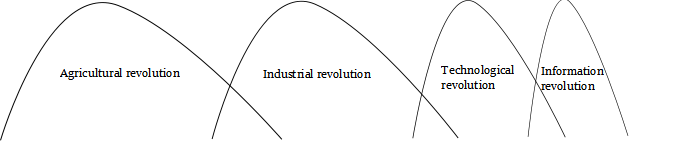
\includegraphics[width=\textwidth]{content/assets/dramagogues--revolution-arcs}
  \end{center}
  \caption{Arcs of revolution}
\end{figure}

Similarly, within our fandom, just as an issue starts to become commonplace (such as the cub-porn ban on FA) or even fade out (such as the Kristal-can't-enjoy-sandwich meme), only a short lull follows before the next surge rockets off from obscurity into brief popularity.  The concept of strife at the dovetail fits at least a little bit here, though it may be a bit of a stretch, as we're not talking about world-wide wars.  Instead, an event such as rumors that PayPal will flag your account if you mention FurAffinity in the message section of your transaction will trigger the next arch, and once that diminishes, we'll switch to perhaps a tracing scandal, or maybe a rumor about Sonic art being banned.

This isn't simply a furry problem, of course, and seems instead to be indicative of those who readily take part in the near-instantaneous forms of communication and new media so prevalent in western culture today.  If we were to take a step back from the furry fandom, I'm sure I could ask similar questions.  Remember the PayPal kerfuffle with Regretsy?  Remember the debt ceiling?  Remember the concerns over the Taepodong missiles?  Heck, even I will admit to having not really thought about SOPA or PIPA much in the last week or two.  In the revolutions graphic above, it's intentional that the arcs become narrower: the amount of time spent dwelling on each of these issues does seem to be growing shorter.

In our so thoroughly connected culture, we've picked up an incredible amount of communication.  It ties us together more thoroughly than any previous era, that's for sure.  On the flip side, however, we have picked up this shorter attention span leading to these more frequent waves of stress and drama.

I don't mean to come off as a get-off-my-lawn, curmudgeonly Luddite.  I did preface that statement with how neat our new-found interconnectedness is, and I am writing this on a website, which will be published to three separate social sites and is powered by free and open-source software -- things I know that I hold dear.  There is, however, a problem in focusing on the extreme near-term with some of these Terribly Important Events.  SOPA started its life a few months ago, but it wasn't until the end of December into the beginning of January that it went viral, leaving it plenty of time to incubate and gain strength.  Additionally, after the house dropped it further bills either cropped up or gained visibility in the mediacentric west such as the OPEN bill and ACTA.  There are, however, root causes to each of these bills, as there are for most such spurts of interest within the media.  Just as online privacy and piracy are the backbone of SOPA, PIPA, OPEN, and ACTA, so too are gender, sexuality, and reproductive rights seemingly the backbones of much of the United States 2012 presidential campaigns.  With that, as interest in the intellectual property bills waned, did interest in online privacy fade as well?  And when the 2012 campaign trail comes to an end, will issues pertaining to gender, sexuality, and reproduction fade from the collective attention span?

That the furry fandom is beginning, in its own way, to exhibit the signs and symptoms shown by the larger culture of western society is indicative of at least two realities.  First, this is a sign that the contiguous fandom is getting large enough to accommodate all of these issues.  The furry subculture has seen a lot of growth in the area of those who identify specifically as furries in the last twenty or thirty years, but most especially in the last ten: we've grown large quickly, and we've started to encompass a variety of issues in our primarily social group.

Secondly, as these issues become more prominent and more prone to ``viral outbreak'', it gets harder to see (and, arguably, more important to remember) that there are individuals at the heart of these Terribly Important Events.  These are the people to whom the events are very important indeed, the ones who will hold onto and remember the moments that passed so quickly through the massed consciousness for a much longer period of time; the ones who care deeply.  However, on the flip side, it's also important to remember that not everyone will react in the same way to what one might consider extremely important.

People, in general, can't hold more than a few things close to their hearts.  It may be difficult to conceive of the fact that something that is of dreadful importance to us is only worth a passing mention to those around us, but rest assured that everyone has their own Terribly Important Events to care about, things that not everyone will have room in their hearts to care about as well.  I've written before about how we're often just like everyone else, and it bears repeating now: we're all just folk here.

That's what so much of this so-called ‘drama' centers around: caring deeply.  Or failing that, caring shallowly but loudly.  An individual may care strongly in either a positive or negative aspect about gender and sexuality issues, to take an example from myself.  But in a community of our size, any individual will not be alone in their focus, having enough many like-minded people around to form a minority sub-community.  In previous articles, as well as in comments here on the site, the concept of minority and majority membership has been brought up: such is the stuff that these arches of drama are made of.  Members caring about something enough to convince others to do the same, if only briefly.
